\chapter{802.15.4 Standard}

Work-group \ac{IEEE} 802.15 was formed to elaborate an standard for the \ac{WPAN}. Inside this work-group, the Task Group 4 
deals with the low binary rate ones, \ac{LR-WPAN}. First standard revision was approved in 2003 with the name of: ``Wireless 
Medium Access Control (MAC) and Physical Layer (PHY) Specifications for Low-Rate Wireless Personal Area Networks (LR-WPANs)'' 
\cite{IEEE802.15.4-2003}.

As it can be observed in the title, the standard defines only the Physical Layer and the \ac{MAC} Layer. Using this base, 
this work will build the Network, Transport and Application Layers to define all network behavior according to the proposed 
High Configurable Protocol.

\section{General Aspects of 802.15.4}

A \ac{LR-WPAN} is a low cost and easy communication network, it allows wireless connection for low binary rate and reduced 
energy consumption applications. This network must provide easy installation, low cost and low energy consumption, it should
also provide a good and reliable data transfer but staying flexible and simple. It cannot be forgotten that as a \ac{WPAN}, it
has a reduced range of work.

\ac{IEEE} 802.15.4 defines the protocol and device interconnection in a \ac{WPAN}, as the objective of this work is not to 
transcribe the standard, only the main characteristics will be presented, focusing later on, just on the important aspects
for this Final Project. To have a deeper view of the standard, refer to \cite{IEEE802.15.4-2003}.

\begin{itemize}
 \item \ac{PHY}: works in 868 MHz (1 ch), 915 MHz (10 ch) and 2450 MHz (16 ch) bands.
 \item Binary rates of 20 kb/s and 40 kb/s at low frequencies and 250 kb/s at 2450 MHz.
 \item Uses 16 bits logic addresses and 64 bits physic addresses.
 \item Possible to use \ac{GTS}.
 \item Channel access through \ac{CSMA/CA}.
 \item \ac{ACK} protocol to assure the communication reliability.
 \item Low consumption oriented.
 \item Provides an Energy Detection system.
 \item Provides a Link Quality Indicator mechanism.
\end{itemize}

Attending to the device functionality, they can be classified in 2 kinds:

\begin{itemize}
 \item \acl{FFD}, this devices have full capacity and functionality, they are the framework of the network. They can connect 
among them but also with other RFD. They are usually plugged in, so energy here will not be a problem. They can provide 
information or act as routers to redirect this information. In every network, there should be one \ac{FFD} who works as \ac{WPAN}
Coordinator, depending on the topology (see Figure \ref{fig:WPAN_Network_Topologies}) all communications must go through the 
Coordinator or not. This Coordinator is usually connected to a central computer that deals with the complexer tasks in the system 
and distributes all the information to the rest of the devices.
 \item \acl{RFD}, this devices have a reduce capacity and functionality as they are thought for easy tasks. This devices are
usually powered with battery and that is why the energy consumption reduction must be focused on them. They can connect only
\ac{FFD} and cannot handle high traffic loads.

\vspace*{1cm}

\begin{figure}[here]
 \begin{center}
  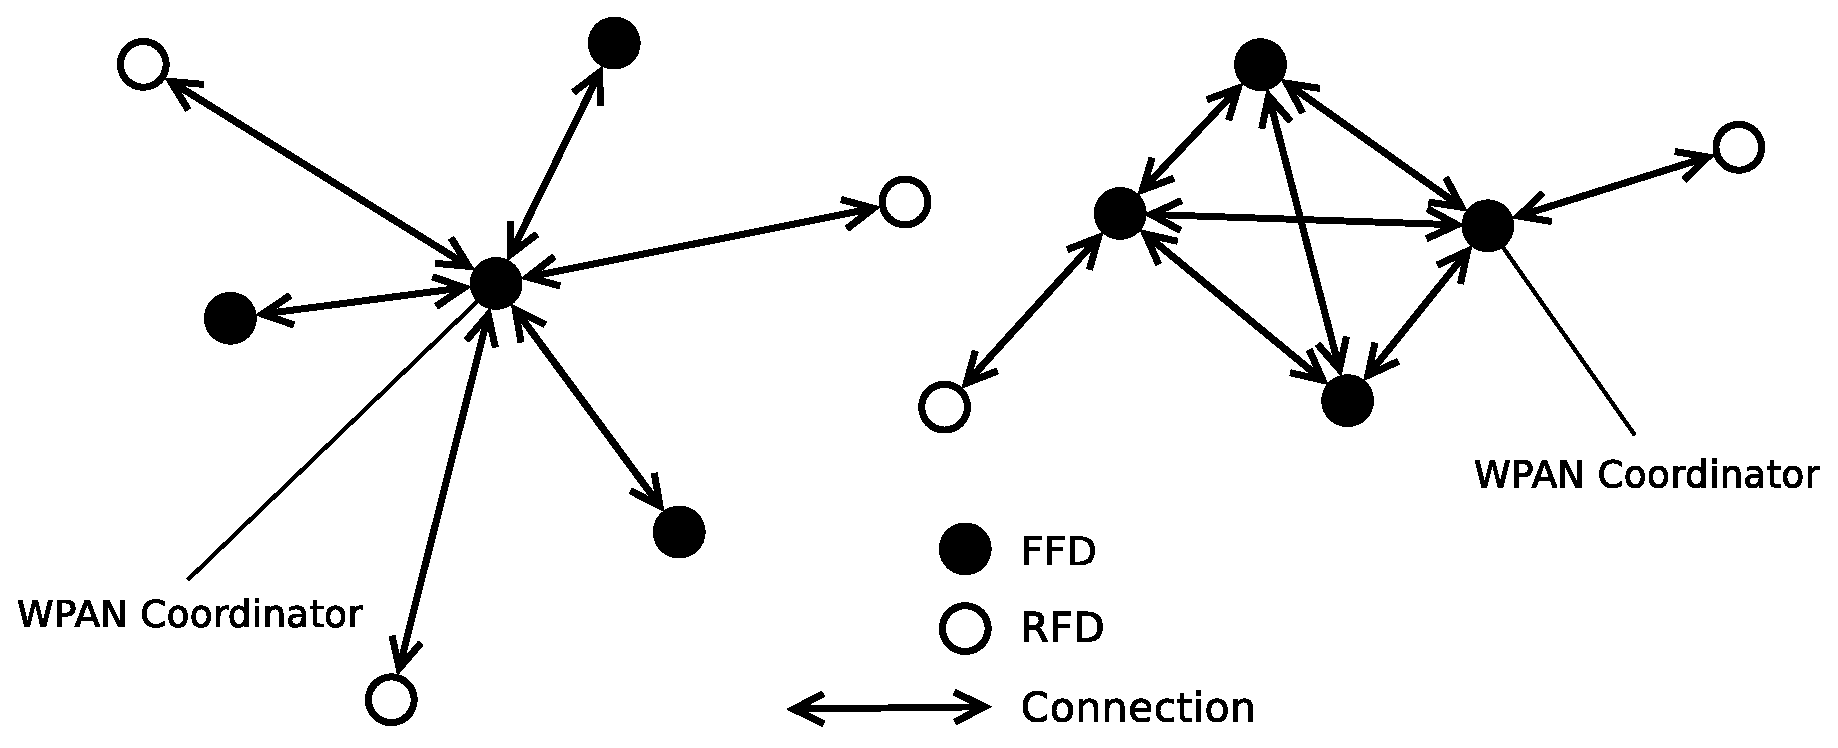
\includegraphics[width=0.9\textwidth]{WPAN_Network_Topologies.eps}
 \end{center}
 \caption{Star and peer-to-peer topology examples \cite{IEEE802.15.4-2003}}
 \label{fig:WPAN_Network_Topologies}
\end{figure}
\end{itemize}
This work will use the peer-to-peer topology as it is more flexible and scalable than the star topology. This topology is also
complexer, that is why a simpler case of peer-to-peer topology is selected, the tree topology. In this case all devices are
structured hierarchically and all of them have a father with whom they communicate, excepting the \ac{WPAN} Coordinator who is on the top of the network.

For this topology, a Network Layer (not provided in 802.15.4) is needed. For routing purposes only the short address (16 bits),
from the 2 kind already commented, will be used. This is to make packets as short as possible.

\section{Physic Layer}

Although for this work \ac{PHY} Layer has not as much importance as the \ac{MAC} Layer, there are some aspects that are important and 
that are good to know. This section will focus just on this aspects.

Some of the tasks developed by the \ac{PHY} Layer are:

\begin{itemize}
 \item \textbf{Switches on and off the radio transceiver.} Transceiver has 3 operation modes, \ac{Tx}, \ac{Rx} and sleeping, \ac{PHY}
layer must commute among this modes by \ac{MAC} layer petition. The standard defines that the change time between \ac{Rx} and 
\ac{Tx} and vice versa cannot be bigger as 12 symbols (\textit{aTurnaroundTime} = 12 symbols = 192 $\mu$s for 2.4 GHz).
 \item \textbf{Performs the \ac{ED} of the channel.} \ac{PHY} layer measures the power level of the channels to choose the best one
to transmit, this measurement lasts exactly 8 symbols.
 \item \textbf{Performs \ac{CCA} to check the channel.} This indicator is a part of \ac{CSMA/CA} algorithm as it will be seen later. The
\ac{CCA} is requested by the \ac{MAC} Layer and the \ac{PHY} Layer returns IDLE or BUSY depending on the channel situation. This \ac{CCA}
period lasts exactly like the \ac{ED}, 8 symbols (128 $\mu$s at 2.4 GHz).
 \item \textbf{Channel frequency selection.} As it was already commented, the 802.15.4 standard contemplates 3 different frequency 
ranges, although this possibility, only the 2450 MHz will be used in this work. At this frequency, the standard stipulates 
the use of a \ac{O-QPSK} modulation with a symbol rate of 62,5 symbol/s. As this modulation makes 4 bit per symbol, we get 
a 250 bit/s bit rate. This frequency range, has 16 different channels with a 5 MHz separation between them, the number of 
this channels goes from 11 to 26.
 \item \textbf{Data transmission and reception.} According to the standard, the \ac{PHY} Layer must be able to transmit with a minimum
power of 1 mW and it must have a sensibility of at least -85 dBm. Figure \ref{fig:PPDU} shows the physical level frame structure.

\vspace*{1cm}

\begin{figure}[here]
 \begin{center}
  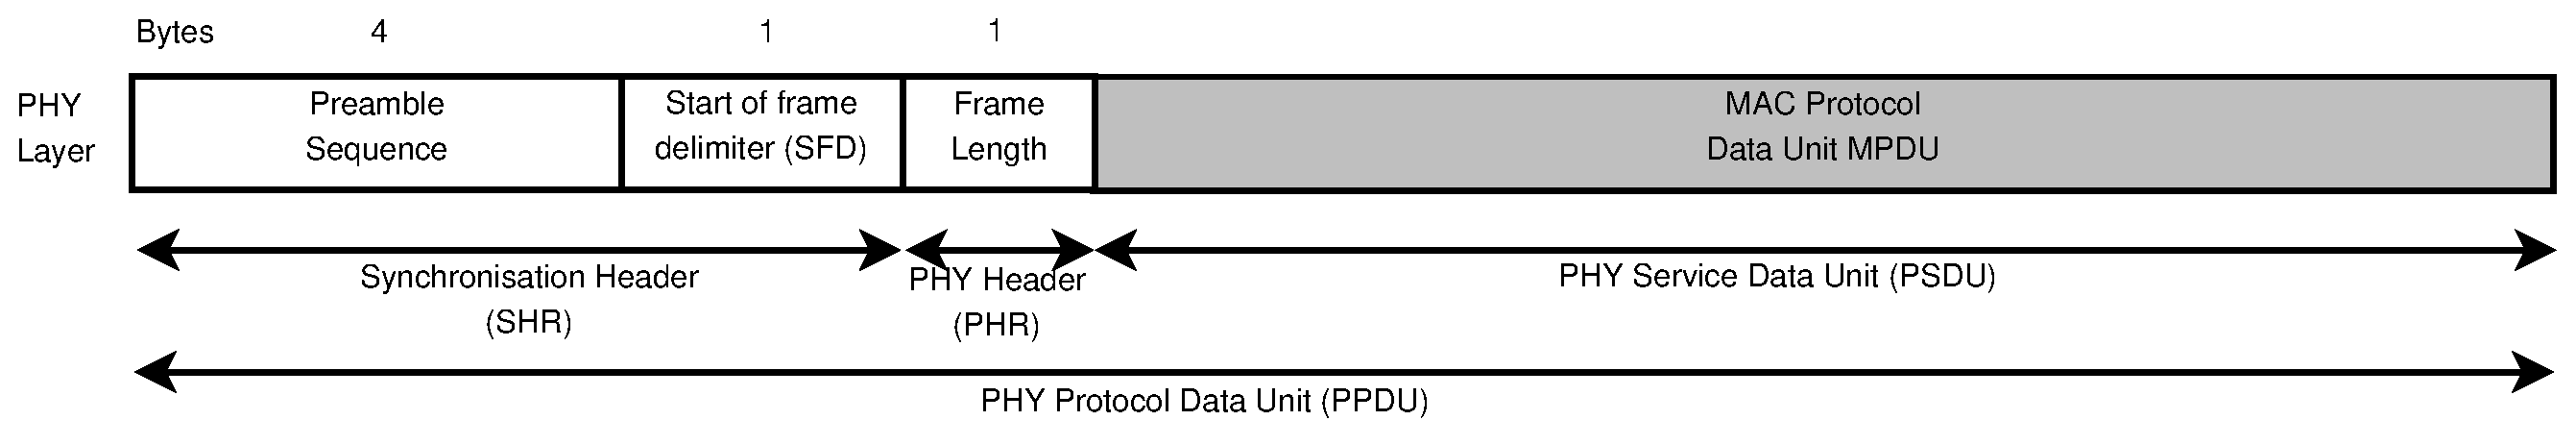
\includegraphics[width=0.9\textwidth]{PPDU.eps}
 \end{center}
 \caption{\ac{PHY} Layer frame \cite{IEEE802.15.4-2003}}
 \label{fig:PPDU}
\end{figure}
\end{itemize}



\section{\ac{MAC} Layer}

Non-Beacon mode as is more flexible for our purposes, but we have to sleep the node manually from the App layer

